
\section{Caesar Salad}
\begin{multicols*}{3}

Place serving bowls and large mixing bowl in the freezer.

\begin{tabular}{r@{ }l}
    \sfrac{1}{2} & loaf rustic bread \\
    \sfrac{1}{2} & stick butter \\
                 & garlic powder (granules) \\
\end{tabular}

Cut bread into ½ inch cubes, sauté  with butter until saturated. Spread on a baking sheet and sprinkle liberally with garlic powder.

Bake at 350 for 10 minutes, and then continue to bake watching closely until golden brown.
Place croûtons in an open container and put in the freezer for 10 minutes.

\begin{tabular}{r@{ }l}
    block parmesan reggiano \\
\end{tabular}

Grate 1 cup coarse, and ½ cup fine.

\begin{tabular}{r@{ }l}
    2 & heads romaine hearts \\
\end{tabular}

Cut into ¾ inch rounds, separate and then chop roughly.

\begin{tabular}{r@{ }l}
    dressing \\
    fresh pepper \\
\end{tabular}

When you're ready to serve, remove large mixing bowl from freezer. Combine lettuce, cheese, pepper and two large spoon fulls of dressing.
Add croûtons, and mix again briefly. Turn out into serving bowls from the freezer.
This must be served immediately. In just a few minutes, the salad will start turning greasy and limp.
Caesar Dressing

\begin{tabular}{r@{ }l}
               1 & large egg \\
               3 & tablespoons lemon juice \\
               1 & teaspoon Worcestershire \\
   1\sfrac{1}{2} & teaspoon anchovy paste \\
               1 &  clove garlic \\
\end{tabular}

Blanch egg in shell for 45 seconds in boiling water. Remove and crack into a small bowl. Whisk with other ingredients.

\begin{tabular}{r@{ }l}
    \sfrac{1}{3} & cup olive oil (extra-virgin) \\
\end{tabular}

Slowly whisk oil into the dressing. Season to taste with salt and pepper.

\end{multicols*}
\clearpage

\newgeometry{margin=0in}
\begin{figure}[p]
    \centering
    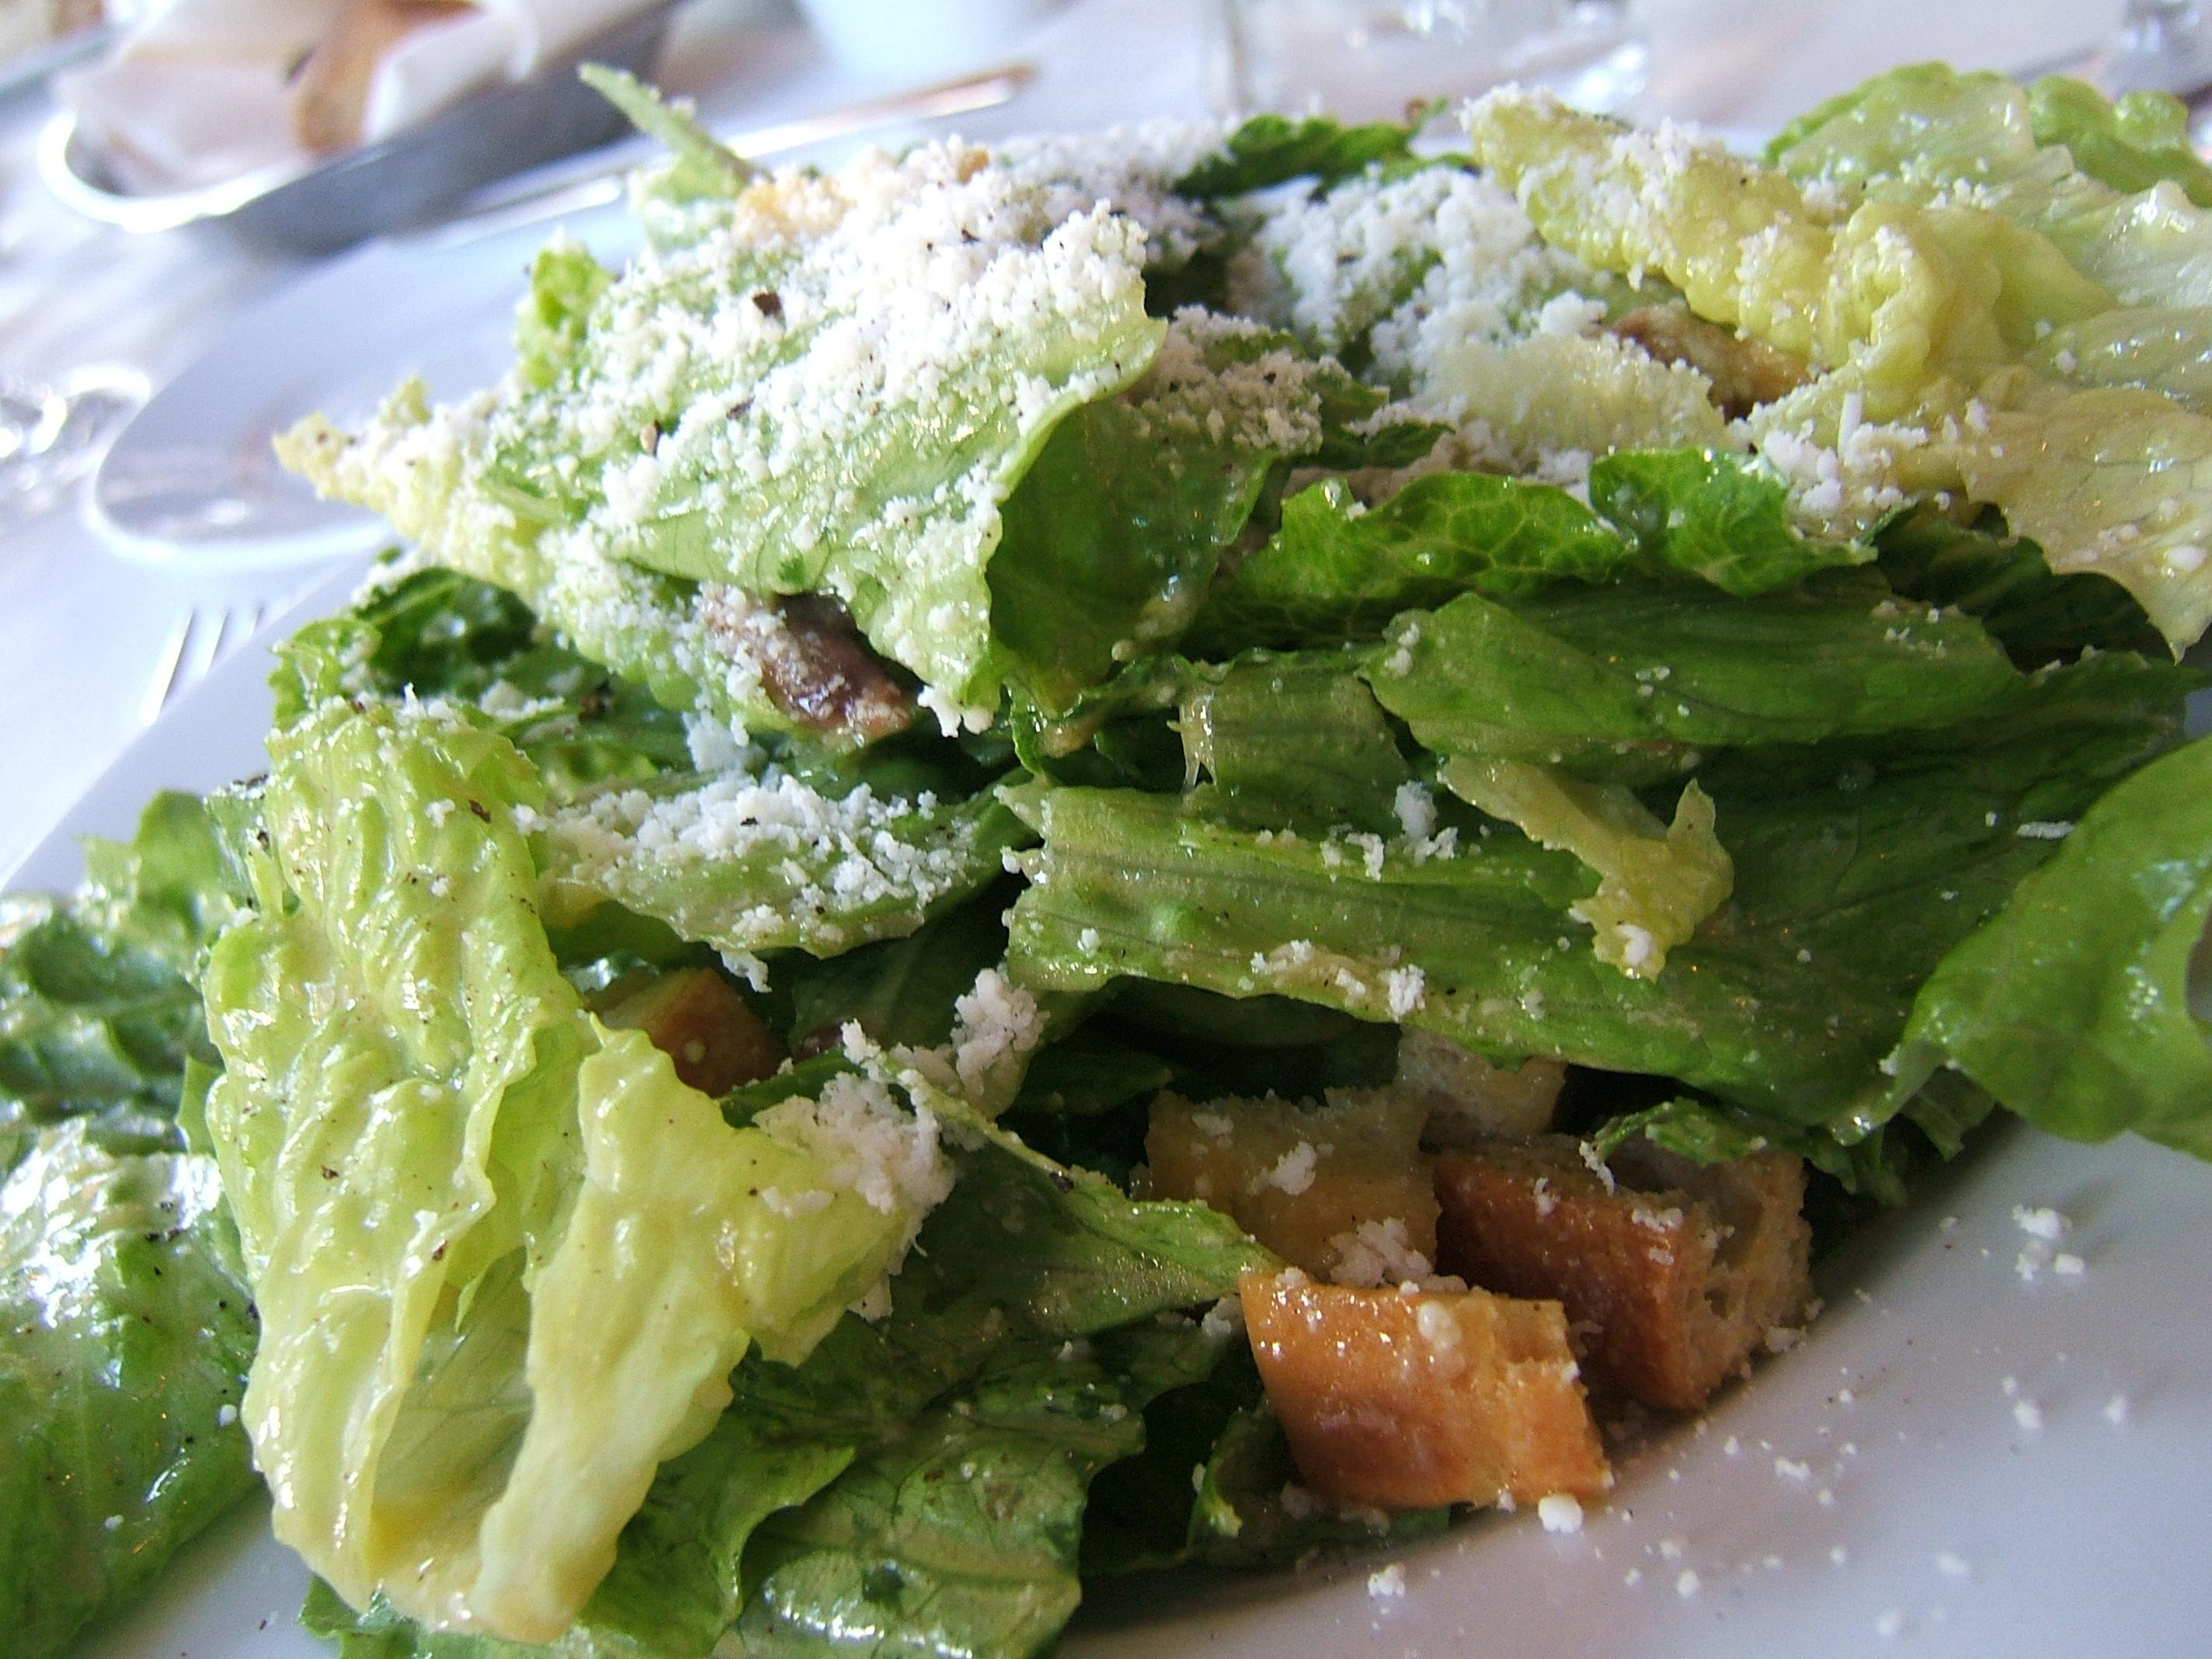
\includegraphics[width=\paperwidth,height=\paperheight]{caesar2.jpg}
    \caption{Caesar Salad}
\end{figure}
\restoregeometry
\clearpage
